
\documentclass[twoside]{article}
\usepackage{../estilo-ejercicios}
\usepackage{enumerate}
\newcommand{\x}{{\mathbf{x}}}
\newcommand{\y}{{\mathbf{y}}}
\usepackage{tikz}
\usetikzlibrary{automata,positioning}
%--------------------------------------------------------
\begin{document}

\title{Procesos Estocásticos. Aplicaciones}
\author{Rafael González López}
\maketitle
\begin{ejercicio}{1} 
Responder a las siguientes cuestiones:
\begin{enumerate}[a)]
\item Definición de cadena de Markov de parámetro continuo.
\item Probar que la definición anterior implque que
\begin{align*}
P[X(t_n)=i_n,\dotsc,X(t_1)=i_1 \mid X(0)=i_0] = \prod_{j=1}^n P[X(t_j) = i_j \mid X(t_{j-1})=i_{j-1}],
\end{align*}
para $0=t_0<t_1<\dotsc<t_n$ y cualesquiera estados $i_j$, $j=0,\dotsc,n$.
\item Utilizando el apartado anterior, probar que un proceso de Poisson es una cadena de Markov de parámetro continuo.
\end{enumerate}
\end{ejercicio}
\begin{solucion}
\begin{enumerate}[a)]
\item[]
\item Una cadena de Markov en tiempo continuo es un proceso estocástico donde $T$, el espacio de parámetros, tiene estructura continua; el espacio de estados tiene estructura discreta, y se cumple la propiedad markoviana, es decir, si $\forall n \geq 2$ $\forall \;0\leq t_1 < \dotsc < t_n$ y $\forall i_0,\dotsc,i_n\in S$ se verifica
$$
P[X(t_n) = i_n \mid X(t_0)=i_0,\dotsc,X(t_{n-1})=i_{n-1}] = P[X(t_n) = i_n \mid X(t_{n-1}) = i_{n-1}]
$$
\item Para $n=2$ tenemos que, por definición
\begin{align*}
P[X(t_2)=i_2,X(t_1)=i_1\mid X(0)=i_0] &= \frac{P[X(t_2)=i_2,X(t_1)=i_1,X(0)=i_0]}{P[X(0)=i_0]}
\end{align*}
Desarrollando el numerador usando la probabilidad condicionada,
\begin{align*}
\frac{P[X(t_2)=i_2\mid X(0)=i_0,X(t_1)=i_1]P[X(t_1)=i_1,X(0)=i_0]}{P[X(0)=i_0]}
\end{align*}
Usando la propiedad markoviana, es equivalente a
$$
\frac{P[X(t_2)=i_2 \mid X(t_1)=i_1]P[X(t_1)=i_1,X(0)=i_0]}{P[X(0)=i_0]}
$$
Finalmente, usando la definición de probabilidad condicionada llegamos al resultado. Supongamos la hipótesis de inducción para $n-1$.
\begin{align*}
P[X(t_n)=i_n,\dotsc,X(t_1)=i_1 \mid X(0)=i_0] &= \frac{P[X(t_n)=i_n,\dotsc, X(0)=i_0]}{P[X(0)=i_0]}
\end{align*}
Expandimos el numerador
\begin{align*}\frac{P[X(t_n)=i_n \mid X(0)=i_0,\dotsc,X(t_{n-1})=i_{n-1}]P[X(t_{n-1})=i_n,\dotsc,X(0)=0]}{P[X(0)=i_0]}
\end{align*}
Al primer factor se le aplica la propiedad markoviana y utilizamos la definición de probabilidad condicionada, obteniendo
$$
P[X(t_n)=i_n\mid X(t_{n-1})=i_{n-1}]P[X(t_{n-1})=i_{n-1},\dotsc,X(t_1)=i_1\mid X(0)=i_0]
$$
Aplicando la hipótesis de inducción al segundo factor obtenemos el resultado.
\item Por definición, un proceso de Poisson es un proceso estocástico en tiempo continuo con espacio de estados discreto con incrementos independientes. Solo hay que probar que tener incrementos independientes implica la propiedad markoviana.
Sean $t_1,\dotsc,t_n$, 
\begin{gather*}
P[T_n =  k_n \mid T_1=k_1,\dotsc,T_{n-1}=k_{n-1}] \\= P[T_n -T_{n-1} =  k_n - k_{n-1}\mid T_1=k_1,\dotsc,T_{n-1}-T_{n-2}=k_{n-1}-k_{n-2}]\\
=P[T_n-T_{n-1}=k_n - k_{n-1}]
\end{gather*}
Ahora bien, volviendo a aplicar incrementos independientes en $t_{n-1},t_n$ tenemos que 
\begin{align*}
P[T_n-T_{n-1}=k_n - k_{n-1}] &= P[T_n -T_{n-1} =k_n - k_{n-1}\mid T_{n-1}  = k_{n-1}]\\
&= P[T_n =k_n \mid T_{n-1} =k_{n-1}]
\end{align*}
\end{enumerate}
\end{solucion}
\newpage

\begin{ejercicio}{2}
Un proceso de Yule es un proceso de nacimiento puro con estados $S=\{1,2,\dotsc\}$, con $\lambda_i=i\lambda$, $i\geq 1$.
\begin{enumerate}[a)]
\item Dibujar el grafo asociado al proceso.
\item Escribir razonadamente la matriz de generadores, $G$, y a partir de la misma describir como evoluciona el proceso.
\item Probar que $P[X(t)=k]=e^{-\lambda t}(1-e^{-\lambda t})^{k-1}$
\item ¿Existe distribución estacionaria?
\end{enumerate}
\end{ejercicio}
\begin{solucion}
\begin{enumerate}[a)]
\item[]
\item El grafo es

\begin{center}
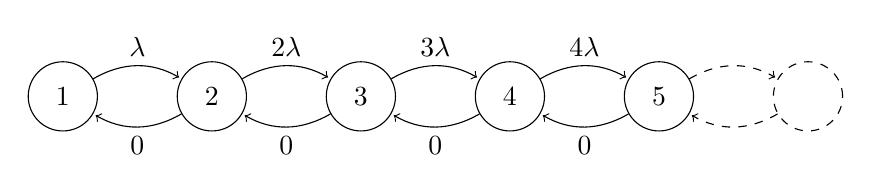
\begin{tikzpicture}
	% Draw the states
	\node[state]             (1) {$1$};
	\node[state, right=of 1] (2) {$2$};
	\node[state, right=of 2] (3) {$3$};
	\node[state, right=of 3] (4) {$4$};
	\node[state, right=of 4] (5) {$5$};
	\node[state, dashed, right=of 5] (6) {$\dotsc$}; 
    % Connect the states with arrows
	\draw[every loop]
		(1) edge[bend left, auto=left] node {$\lambda$} (2)
		(2) edge[bend left, auto=left] node {$0$} (1)
		(2) edge[bend left, auto=left] node {$2\lambda$} (3)
		(3) edge[bend left, auto=left] node {$0$} (2)
		(3) edge[bend left, auto=left] node {$3\lambda$} (4)
		(4) edge[bend left, auto=left] node {$0$} (3)
		(4) edge[bend left, auto=left] node {$4\lambda$} (5)
		(5) edge[bend left, auto=left] node {$0$} (4)
		(5) edge[bend left, auto=left, dashed] node {} (6)
		(6) edge[bend left, auto=left, dashed] node {} (5);
;
\end{tikzpicture} 
\end{center}
\item La matriz asociada es
$$
G= 
\begin{pmatrix}
-\lambda & \lambda & 0 &  \cdots & 0 & 0 & 0 & \cdots \\
0 & -2\lambda & 2\lambda &  \cdots& 0 & 0 & 0 &\cdots \\
0 & 0 & -3\lambda & \cdots & 0 & 0 & 0 &\cdots \\
\vdots & \vdots& \vdots & & \vdots & \vdots & \vdots\\
0 & 0 & 0 & \cdots & -i\lambda & i \lambda & 0 & \cdots\\
\vdots & \vdots & \vdots & & \vdots & \vdots & \vdots
\end{pmatrix}
$$
Tenemos un proceso de nacimiento lineal sin muerte. Lo único que puede ocurrir es que nos quedemos en el estado actual o aumentar la cantidad de individuos, lo cuál es la cada vez más probable.
\item Sea $\rho_k(t) = P[X(t)=k]$, tenemos que $\rho_t'=\rho_t G$. Sabemos que $\rho_k(0)=1$. Tenemos 
\begin{align*}
\rho_1(t)' = -\rho_1(t)\lambda \Rightarrow \rho_1(t)=e^{-\lambda t}
\end{align*}
$$
\rho_k(t)' = (k-1)\lambda\rho_{k-1}(t)-k\lambda\rho_k(t)
$$
Vamos a probar el resultado por inducción. Para $k=1$ ya lo tenemos, $\rho_1(t)=e^{-\lambda t}$. Supongamos que es cierto para $k-1$. Entonces, aplicando la hipótesis de inducción a la ecuación diferencial
$$
\rho_k(t)' = (k-1)\lambda e^{-\lambda t}(1-e^{-\lambda t})^{k-2}-k\lambda\rho_k(t)
$$
La solución general de dicha ecuación es
$$
Ce^{-k\lambda t} + e^{-\lambda t}(1-e^{-\lambda t})^{k-1}
$$
Imponiendo que $\rho_k(0)=1$ (y dado que $k\geq 2$) obtenemos que $C=0$. 
\item Comprobemos primero la ecuación $\pi G=0$.
$$
\pi G = 0 \Leftrightarrow -\pi_1 \lambda  = 0 \text{ y } i\pi_i \lambda - (i+1)\lambda \pi_{i+1} = 0
$$
Dado que $i\lambda > 0$, tenemos que $\pi_1 = 0$. Por inducción es claro que $\pi_i = 0$ $\forall i$, por lo que no existe distribución estacionaria.
\end{enumerate}
\end{solucion}



\newpage

\begin{ejercicio}{3}
Sea $X(t)$ un proceso de nacimiento y muerte con estados $S=\{0,1,\dotsc\}$, con $\lambda_i = \lambda$, $i\geq 0$ y $\mu_i = \mu $ $i\geq 1$ $(\mu_0 = 0)$.
\begin{enumerate}[a)]
\item Dibujar el grafo asociado al proceso.
\item Escribir razonadamente la matriz de generadores, $G$ y a partir de la misma describir como evoluciona el proceso.
\item Bajo qué condiciones para $\lambda$ y $\mu$ existe distribución estacionaria.
\item En caso de que exista una distribución estacionaria calcular $\lim_{t\to \infty}P[X(t)=k]$, ¿cuánto vale ese límite si no hay distribución estacionaria?
\end{enumerate}
\end{ejercicio}
\begin{solucion}
\begin{enumerate}[a)]
\item[]
\item El grafo asociado es

\begin{center}
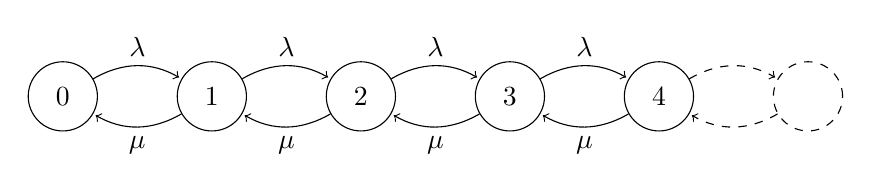
\begin{tikzpicture}
	% Draw the states
	\node[state]             (1) {$0$};
	\node[state, right=of 1] (2) {$1$};
	\node[state, right=of 2] (3) {$2$};
	\node[state, right=of 3] (4) {$3$};
	\node[state, right=of 4] (5) {$4$};
	\node[state, dashed, right=of 5] (6) {$\dotsc$}; 
    % Connect the states with arrows
	\draw[every loop]
		(1) edge[bend left, auto=left] node {$\lambda$} (2)
		(2) edge[bend left, auto=left] node {$\mu $} (1)
		(2) edge[bend left, auto=left] node {$\lambda$} (3)
		(3) edge[bend left, auto=left] node {$\mu$} (2)
		(3) edge[bend left, auto=left] node {$\lambda$} (4)
		(4) edge[bend left, auto=left] node {$\mu$} (3)
		(4) edge[bend left, auto=left] node {$\lambda$} (5)
		(5) edge[bend left, auto=left] node {$\mu$} (4)
		(5) edge[bend left, auto=left, dashed] node {} (6)
		(6) edge[bend left, auto=left, dashed] node {} (5);
;
\end{tikzpicture} 
\end{center}
\item La matriz asociada es
$$
G= 
\begin{pmatrix}
-\lambda & \lambda & 0 &  \cdots & 0 & 0 & 0 & \cdots \\
\mu & -(\lambda + \mu) & \lambda &  \cdots& 0 & 0 & 0 &\cdots \\
0 & \mu & -(\lambda + \mu)  & \cdots & 0 & 0 & 0 &\cdots \\
0 & 0 &  \mu & \cdots & 0 & 0& 0 & \cdots\\
\vdots & \vdots& \vdots & & \vdots & \vdots & \vdots\\
0 & 0 & 0 & \cdots & \mu  & -(\lambda +  \mu) & \lambda & \cdots\\
\vdots & \vdots & \vdots & & \vdots & \vdots & \vdots
\end{pmatrix}
$$
Es claro que el proceso es de la siguiente manera. Si partimos de un estado $i$, solo podemos pasar a tener un individuo más en el grupo, o esperar que alguno de los ya existentes muera. 
\item Sabemos por teoría que si existe la distribución estacionaria, entonces $\pi G  = 0$. Si $\mu \neq 0$, entonces
$$
\pi_k = \frac{\lambda_0 \cdots \lambda_{k-1}}{\mu_1 \cdots \mu_n }\pi_0 = \frac{\lambda^k}{\mu^k}\pi_0
$$
Tenemos que imponer que la suma sea $1$, luego
$$
1 =  \pi_0 \sum_{k=0}^\infty \frac{\lambda^k}{\mu^k } = \pi_0 \frac{1}{1-\lambda/\mu}
$$
Por tanto, $\pi_0 = 1-\lambda/\mu$. Dado que $\lambda,\mu \geq 0$, basta imponer que $\lambda \leq \mu$. Si $\mu = 0$ entonces tenemos un proceso de nacimiento sin muerte. En este último caso, claramente no hay distribución estacionaria.
\item Por teoría, sabemos que si existe la distribución estacionaria
$$
P[X(t)=k] \rightarrow \pi_k = \frac{\lambda^k}{\mu^k}(1-\lambda/\mu)
$$
En otro caso, el límite es $0$.
\end{enumerate}
\end{solucion}
\end{document}